\subsection{The standard Kyle market: low trading without punishment}
\label{sec:kyle}

Table~\ref{tab:core} and Figure~\ref{fig:core} report outcomes for two
learners in the standard Kyle market ($\xi=0$) with a constant step size
$\alpha=0.15$, 200 markets per seed and three seeds per condition.

\paragraph{Outcomes.} Forward-looking learners that remember what their rivals
and the noise traders did (\emph{residual} memory) trade far below Nash: their
aggregate intensity covers $\ResidDeltaInt$ of the distance from competition to
the cartel (seed means \ResidSeedRange), informativeness $\ResidDeltaInfo$,
and profit $\ResidDeltaProfit$. With perfect monitoring of each other's
orders, the index is $\OrdersDeltaInt$. Without memory, where punishment is
impossible, learners still close $\NoneDeltaInt$ of the gap. Read
conventionally, these numbers describe substantial collusion.

\paragraph{The myopic placebo.} Retraining the residual-memory learners with
$\gamma=0$, which removes any reason to punish or to fear punishment, produces
an intensity index of $\MyopicResidDeltaInt$ and an informativeness index of
$\MyopicResidDeltaInfo$: myopic learners trade \emph{less than the cartel} and
make prices less informative than full collusion would. They do not, however,
earn collusive profits ($\Delta$ profit $=\MyopicResidDeltaProfit$), because
trading below the cartel level gives up profit. A learner that cannot collude
thus scores higher on the intensity- and informativeness-based indices than
learners that might. These indices measure how little algorithms trade, not
why, and cannot by themselves identify collusion.

\paragraph{Punishment tests.} The rival-deviation test is the most direct evidence.
Figure~\ref{fig:deviation} shows that after a forced one-period best-response
deviation, rivals' trading intensity is unchanged at every lag in every
condition: the reaction at the first lag is $\ResidRivalLagOne\pm\ResidRivalLagOneCI$
for residual memory and $\OrdersRivalLagOne\pm\OrdersRivalLagOneCI$ (about
$\OrdersReactionPct$\% of the deviation itself) with perfect monitoring.
Deviating pays: the deviator's discounted gain over the following 16 periods is
$\ResidGain\pm\ResidGainCI$ with residual memory and
$\OrdersGain\pm\OrdersGainCI$ with perfect monitoring, essentially all of it
earned in the deviation period. No condition shows the
punishment-then-reversion pattern that identifies collusion in
\citet{calvano2020}. The outcome is supracompetitive but not
self-enforcing, which is the signature of pruning.

This matches Proposition~\ref{prop:snr}: at $\xi=0$ a best-response deviation
is about a quarter of a noise standard deviation per unit of $v/\sigma_v$, so
a trigger on observed flow would fire mostly on noise. It is also consistent with the classification of \citet{dou2025}, as reported in
their reimplementation \citep{esquinas2026}, which attributes collusion at $\xi=0$
to over-pruning. What our diagnostics add is that even perfect monitoring, which
removes the detectability problem entirely, does not lead Q-learners to
discover punishment.

\paragraph{Convergence.} With a constant step size and noisy payoffs, greedy
strategies keep changing among neighbouring orders: on-path orders moved by
$\ResidShift$ grid steps on average over the last $10^5$ training periods
(residual memory). Outcomes are nevertheless stable: seed-to-seed variation
in $\Delta$ is a few hundredths, and the residual-memory results are unchanged
between $6\times10^6$ and $1.5\times10^7$ training periods (Appendix
Table~\ref{tab:robust}).

\begin{table}[t]
  \centering
  \small
  \resizebox{\linewidth}{!}{\begin{tabular}{lccccccc}
\toprule
Condition & $\Delta$ intensity & $\Delta$ inform. & $\Delta$ profit & Rival $\Delta\beta_1$ & $\Delta\beta_1/\Delta\beta^{\mathrm{dev}}_0$ & Deviator gain & Markets \\
\midrule
Remembers rivals ($\gamma=0.95$) & $0.86 \pm 0.01$ & $0.93 \pm 0.01$ & $0.46 \pm 0.02$ & $-0.000 \pm 0.003$ & $-0.00$ & $0.053 \pm 0.003$ & 600 \\
Remembers rivals, myopic ($\gamma=0$) & $1.241 \pm 0.005$ & $1.46 \pm 0.01$ & $-0.01 \pm 0.01$ & $0.002 \pm 0.003$ & $0.00$ & $0.124 \pm 0.004$ & 600 \\
No memory ($\gamma=0.95$) & $0.24 \pm 0.02$ & $0.26 \pm 0.02$ & $0.16 \pm 0.04$ & $0.000 \pm 0.000$ & $0.00$ & $0.018 \pm 0.001$ & 600 \\
No memory, myopic ($\gamma=0$) & $1.27 \pm 0.03$ & $1.49 \pm 0.03$ & $-0.03 \pm 0.05$ & $0.000 \pm 0.000$ & $0.00$ & $0.115 \pm 0.003$ & 600 \\
Perfect monitoring ($\gamma=0.95$) & $0.82 \pm 0.01$ & $0.90 \pm 0.01$ & $0.39 \pm 0.03$ & $0.008 \pm 0.008$ & $0.03$ & $0.058 \pm 0.007$ & 200 \\
\bottomrule
\end{tabular}}
  \caption{Standard Kyle market ($\xi=0$, $I=2$, constant $\alpha=0.15$).
  $\Delta$: collusion indices (0 = Nash, 1 = cartel) pooled over markets and
  seeds. Rival $\Delta\beta_1$: change in rivals' trading intensity one period
  after a forced best-response deviation; next column: the same as a fraction
  of the deviation. Deviator gain: discounted profit gain from deviating over
  16 periods. 95\% confidence intervals.}
  \label{tab:core}
\end{table}

\begin{figure}[t]
  \centering
  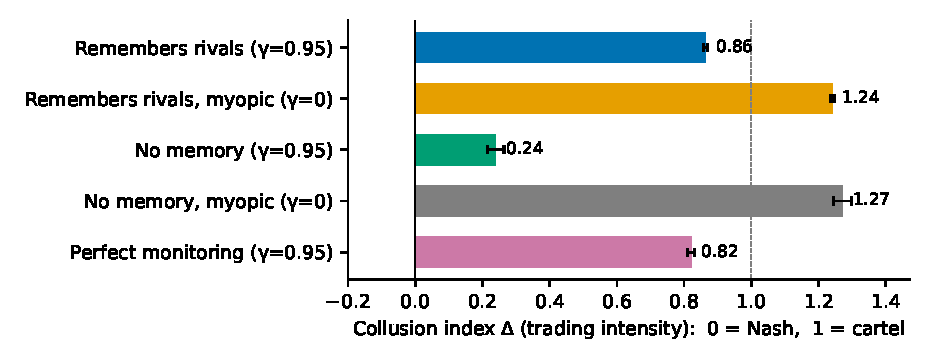
\includegraphics[width=0.8\linewidth]{figures/fig_core.pdf}
  \caption{Collusion index (trading intensity) by condition. The myopic
  placebo, which cannot collude, scores beyond the cartel.}
  \label{fig:core}
\end{figure}

\begin{figure}[t]
  \centering
  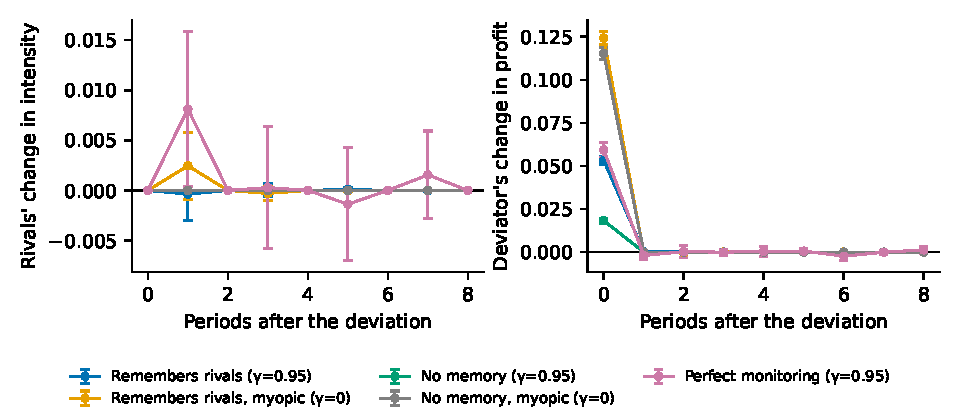
\includegraphics[width=0.9\linewidth]{figures/fig_deviation.pdf}
  \caption{Rival-deviation test. Left: change in rivals' trading intensity
  after trader~1 plays its one-period best response at lag 0. Right: the
  deviator's change in profit. Paired simulations with common random numbers;
  95\% confidence intervals.}
  \label{fig:deviation}
\end{figure}
